%%%% Better Poster latex template example v1.0 (2019/04/04)
%%%% GNU General Public License v3.0
%%%% Rafael Bailo
%%%% https://github.com/rafaelbailo/betterposter-latex-template
%%%% 
%%%% Original design from Mike Morrison
%%%% https://twitter.com/mikemorrison

\documentclass[]{betterposter}
\geometry{paperwidth=39in,paperheight=39in}
%%%% Uncomment the following commands to customise the format


%% Setting the width of columns
% Left column
\setlength{\leftbarwidth}{0.25\paperwidth}
% Right column
%\setlength{\rightbarwidth}{0.25\paperwidth}

%% Setting the column margins
% Horizontal margin
%\setlength{\columnmarginvertical}{0.0002\paperheight}
% Vertical margin
\setlength{\columnmarginhorizontal}{0.01\paperheight}
% Horizontal margin for the main column
\setlength{\maincolumnmarginvertical}{0.05\paperheight}
% Vertical margin for the main column
%\setlength{\maincolumnmarginhorizontal}{0.03\paperheight}

%% Changing font sizes
% Text font
%\renewcommand{\fontsizestandard}{\fontsize{28}{35} \selectfont}
% Main column font
%\renewcommand{\fontsizemain}{\fontsize{28}{35} \selectfont}
% Title font
%\renewcommand{\fontsizetitle}{\fontsize{28}{35} \selectfont}
% Author font
%\renewcommand{\fontsizeauthor}{\fontsize{28}{35} \selectfont}
% Section font
%\renewcommand{\fontsizesection}{\fontsize{25}{32} \selectfont}

%% Changing font sizes for a specific text segment
% Place the text inside brackets:
% {\fontsize{28}{35} \selectfont Your text goes here}

%% Changing colours
% Background of side columns
%\renewcommand{\columnbackgroundcolor}{black}
% Font of side columns
%\renewcommand{\columnfontcolor}{gray}
% Background of main column
%\renewcommand{\maincolumnbackgroundcolor}{yellow}
%\renewcommand{\maincolumnbackgroundcolor}{theory}
%\renewcommand{\maincolumnbackgroundcolor}{methods}
%\renewcommand{\maincolumnbackgroundcolor}{intervention}
% Font of main column
%\renewcommand{\maincolumnfontcolor}{gray}

\begin{document}	



\betterposter{
%%%%%%%% MAIN COLUMN

\maincolumn{
%%%% Main space
\begin{flushleft}
\textbf{Concentration} and \textbf{sleep} are more central when depression in PTSD is accounted for.
%Higher centrality of \textbf{concentration} and \textbf{sleep} symptoms when \textbf{depression} in PTSD is accounted.
\end{flushleft}


\null
%\vfill
\begin{center}
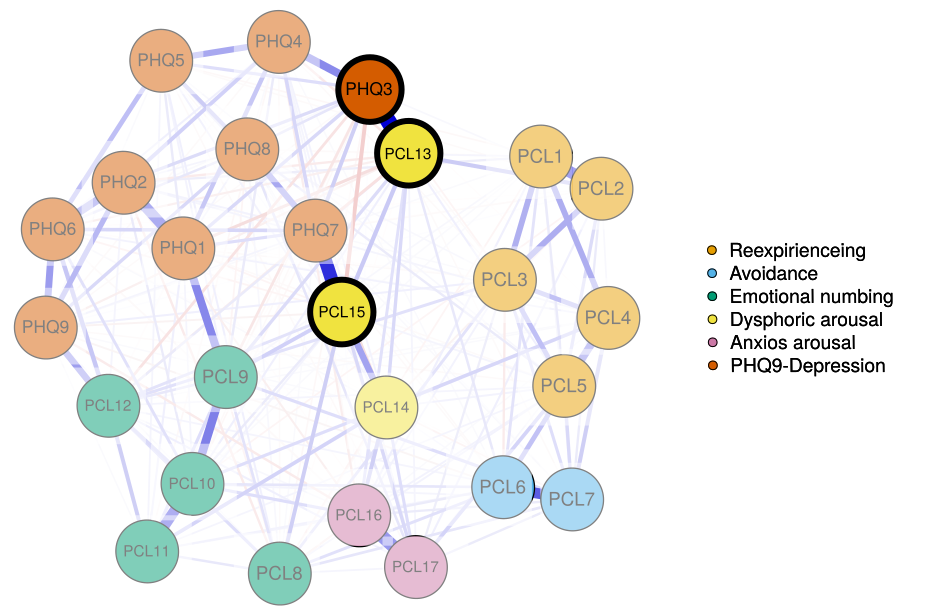
\includegraphics[scale=1.5]{img/opaqueNetwork.png}    
\end{center}

}{
%%%% Bottom space
%% QR code
\qrcode{img/qrcode.png}{img/smartphoneWhite}{
\textbf{Take a picture} to \\
download the full poster
}
{
\begin{flushright}

\includegraphics[width=0.04\textwidth]{img/twitter.png}
@orduek
\end{flushright}
}
% Smartphone icon
% Author: Freepik
% Retrieved from: https://www.flaticon.com/free-icon/smartphone_65680

%% Compact QR code (comment the previous command and uncomment this one to switch)
%\compactqrcode{img/qrcode}{
%\textbf{Take a picture} to
%\\download the full paper
%}

}

}{
%%%%%%%% LEFT COLUMN

\title{Concentration and \\ Sleep in PTSD}
\author{Duek, Or}
\author{Hoff, Ranni}
\author{Harpaz-Rotem Ilan}

\institution{Yale University School of Medicine}
\institution{National Center for PTSD}

\section{Introduction}
\begin{itemize}
\item Importance of core symptoms in PTSD is still debatable
\item Past network-approach studies used small/medium sample size
\item More emphasis on\\ comorbidity in PTSD, especially depression
\item Network-approach $\rightarrow$ understand relations between different symptoms
\end{itemize}

\section{Method}
\begin{itemize}
\item Data collected from DoD/VA
\item Analyzed only PTSD symptoms [PCL-4,(N=159,577)]
\item Analyzed PTSD with Depression symptoms [PCL-4\&PHQ9, (N=33,088)]
\item Used directed acyclic graph (DAG) to find \\directionality in the network
\end{itemize}


\section{Results}
\begin{itemize}
    \item Only PTSD $\rightarrow$ higher centrality of trauma\\ related symptoms
    \item PTSD with depression $\rightarrow$ Higher centrality of sleep \& concentration symptoms
    \item DAG $\rightarrow$ Intrusion leads to other symptoms
\end{itemize}

\begin{center}
\textbf{Centrality of PTSD alone \& PTSD and Depression}
    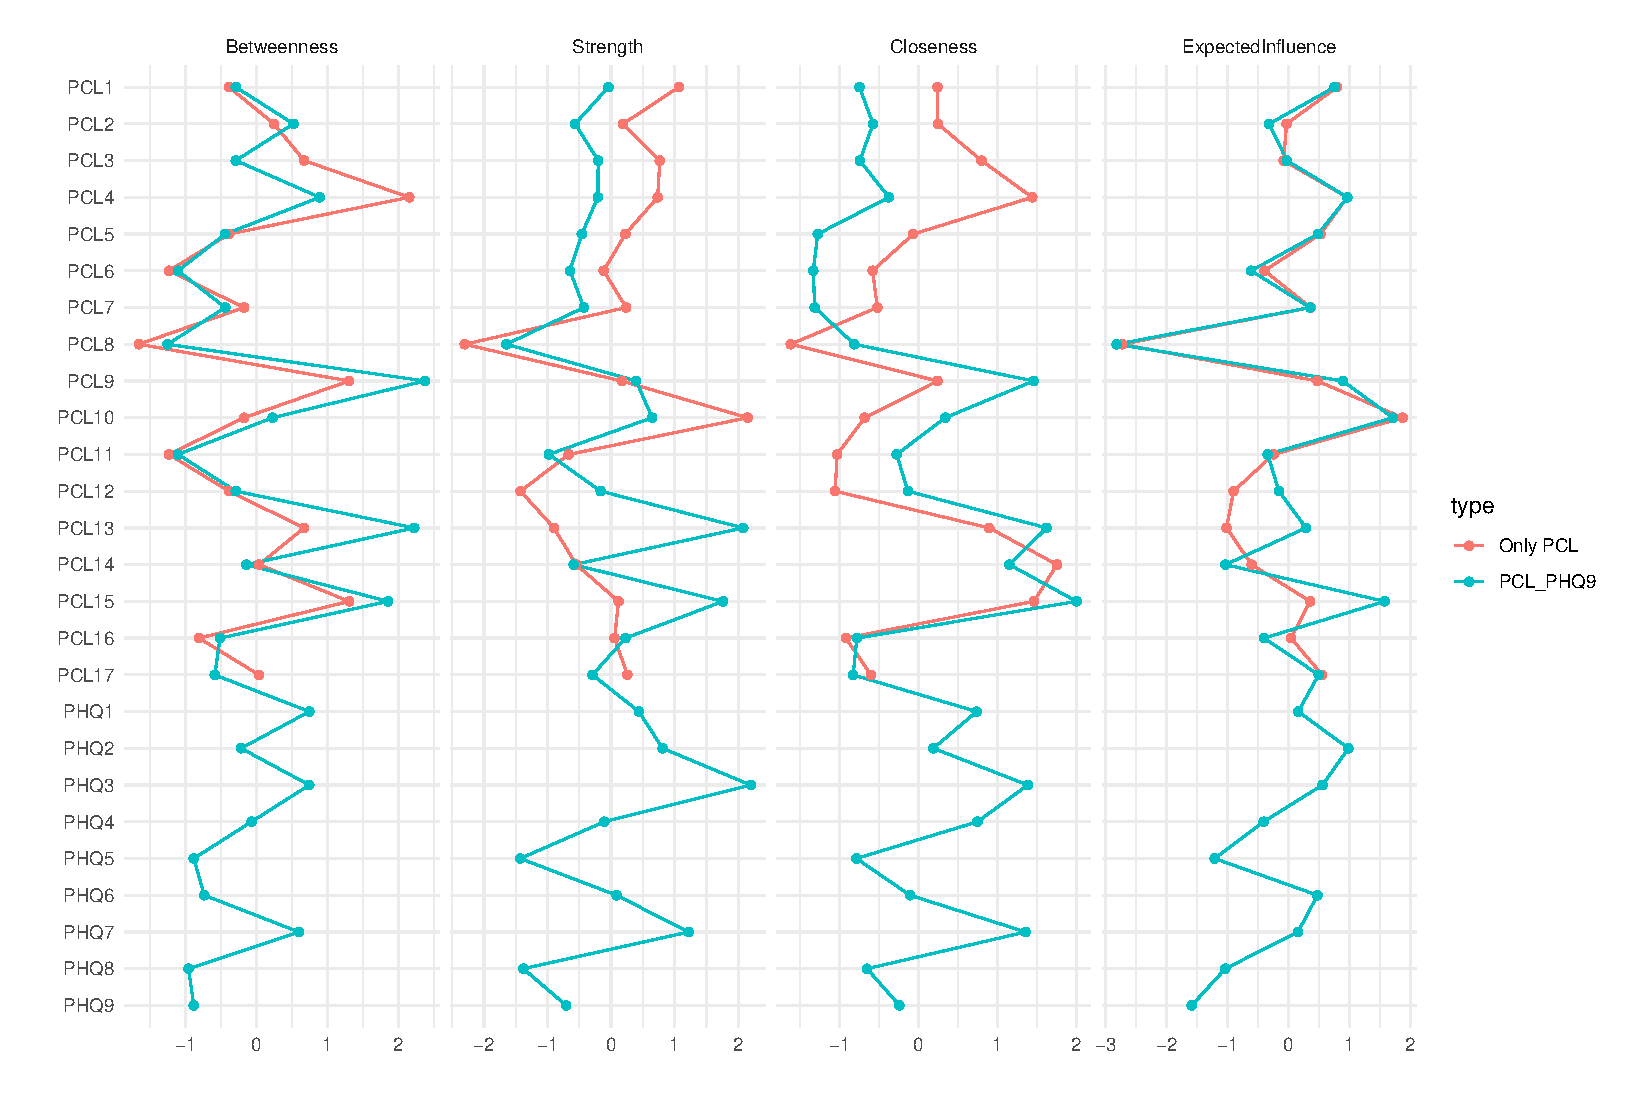
\includegraphics[width=0.99\textwidth, height=0.7\textwidth]{img/centralityTotal.eps}
\end{center}

\section{Conclusion}
\begin{itemize}
    \item Sleep and concentration are very important in PTSD with comorbid depression
    \item Might affect our clinical intervention in the future (more focus on sleep \& concentration)
\end{itemize}

%% This fills the space between the content and the logo
\vfill

%% Institution logo
% \begin{center}


% 
\includegraphics[width=0.3\textwidth]{img/yalesm.png}\\
% \end{center}
}{
%%%%%%%% RIGHT COLUMN

\section{}
\section{Network Graphs}

Graph describes the partial correlation (LASSO) between PCL alone (1$^{st}$) or PCL and PHQ9 (2$^{nd}$) symptoms
(five clusters\\ according to $^{(Harpaz-Rotem \ et al. 2014)}$ \\ % fix space here
Stronger correlations are presented using higher saturation and wider lines
\begin{center}
% Commutative diagram with edges passing under/over
% Author: Stefan Kottwitz, http://texblog.net/
% Retrieved from: http://www.texample.net/tikz/examples/commutative-diagram/
\textbf{PTSD symptoms}
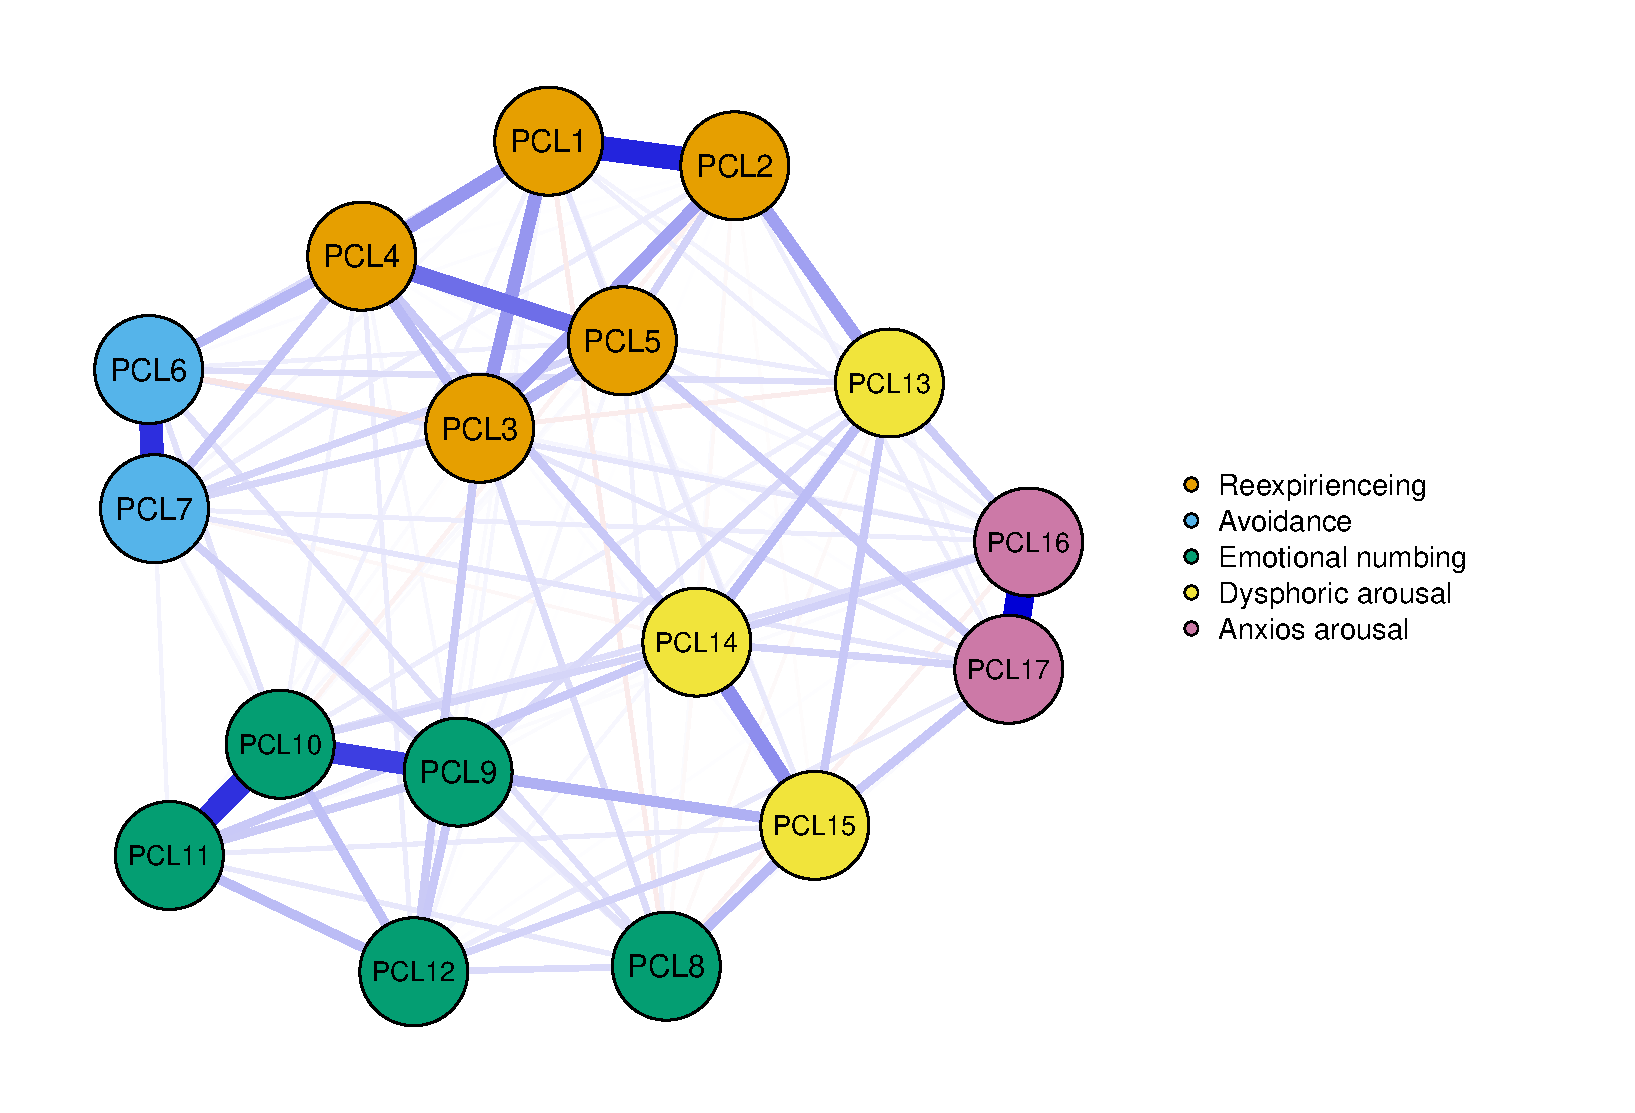
\includegraphics[width=\textwidth]{img/pclOnlyNetwork.eps}
\end{center}
\\

\\
\begin{center}
\textbf{PTSD \& Depressive symptoms}
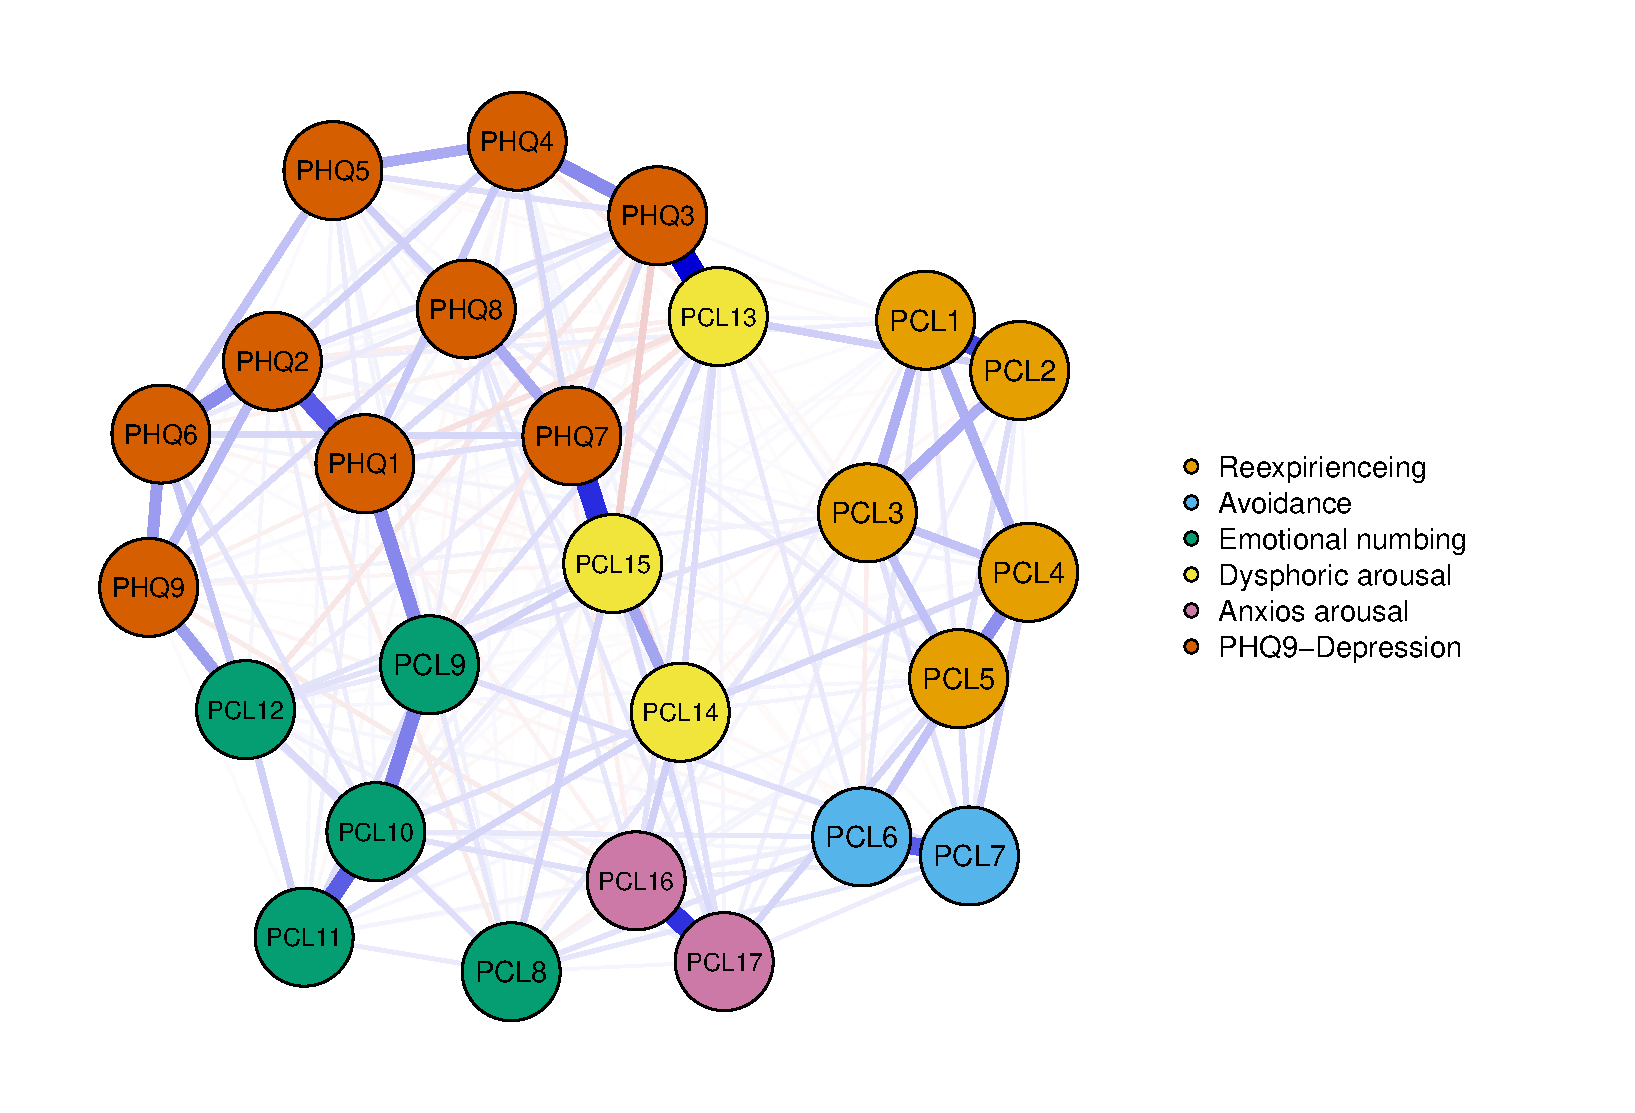
\includegraphics[width=\textwidth]{img/PCL_PHQ9Network.eps}
\end{center}

\section{DAG}
\begin{center}
Directed acyclic graph reveals intrusive thoughts as most pivotal
\begin{SCfigure}
    \centering
    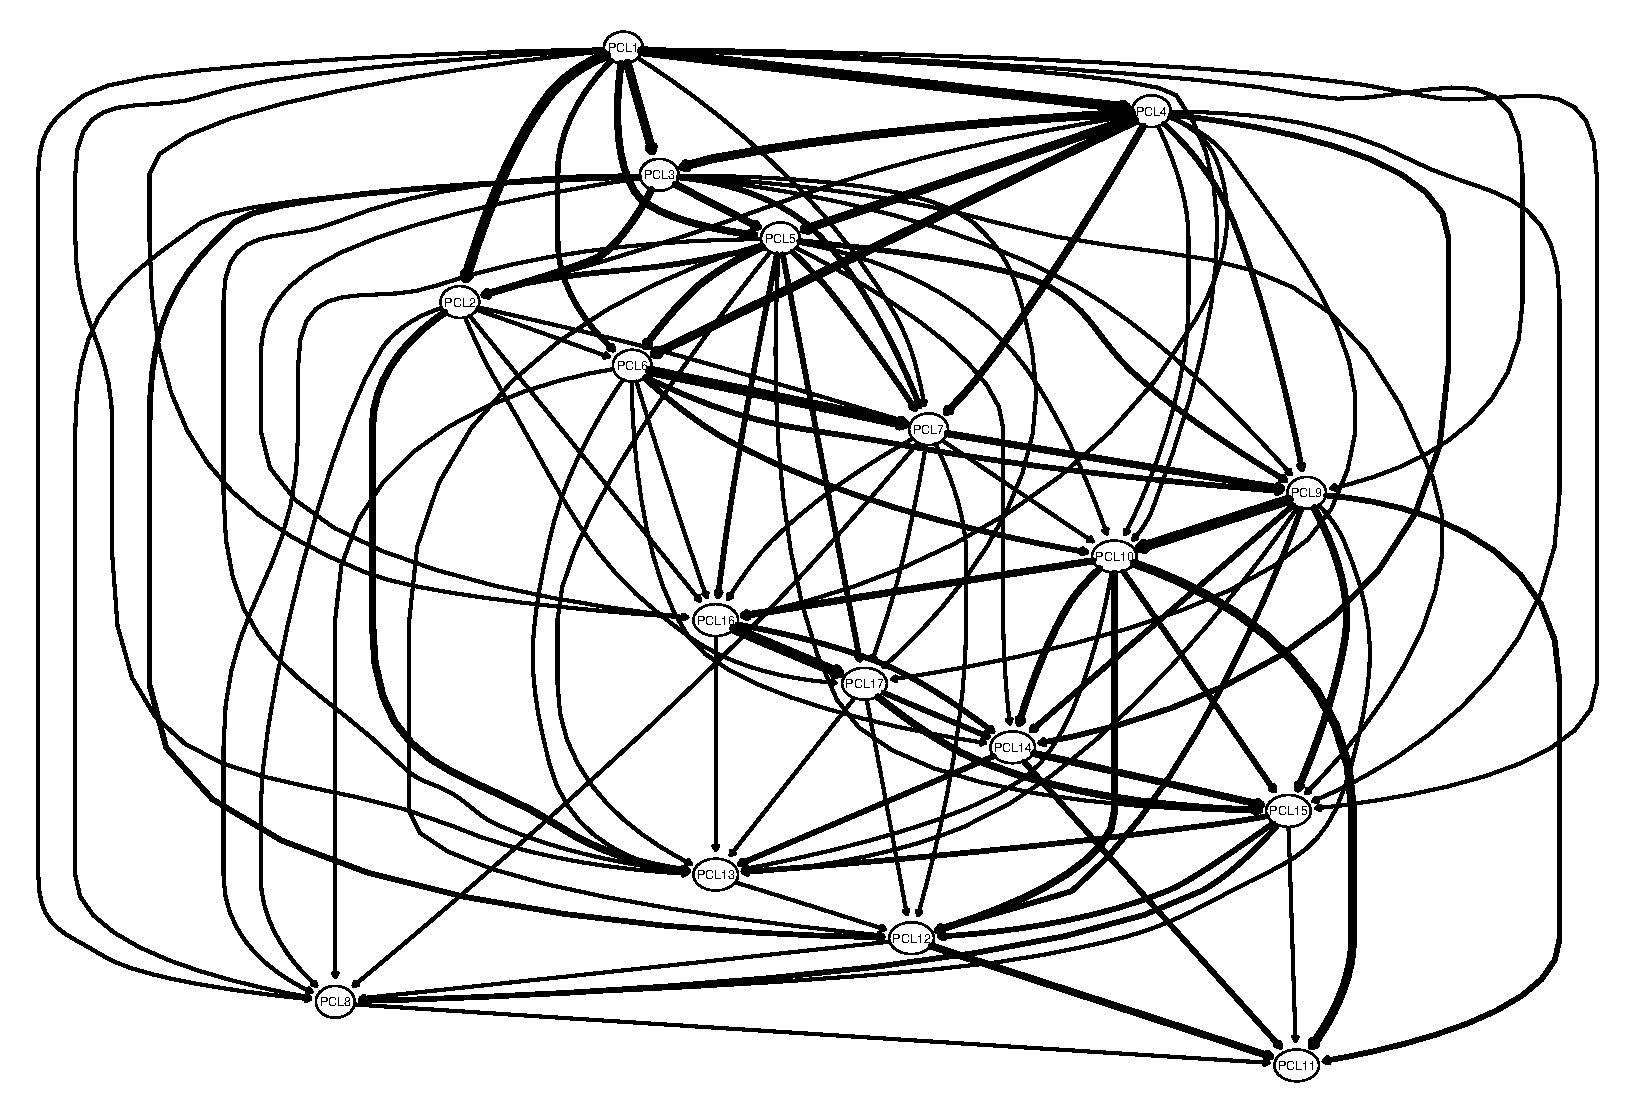
\includegraphics[width=\textwidth, height=1.05\textwidth]{img/pcl_DAG.eps}
    %\caption{Figure present directionality of symptom's correlation}
    \label{fig:my_label}
\end{SCfigure}
    %\includegraphics
    %\caption{[width=0.5\textwidth]}
\end{center}
%\section{Difference}
%\begin{center}
%This is a graph example of difference between the two networks. Depression symptoms explain 6.3\% of connectivity
%    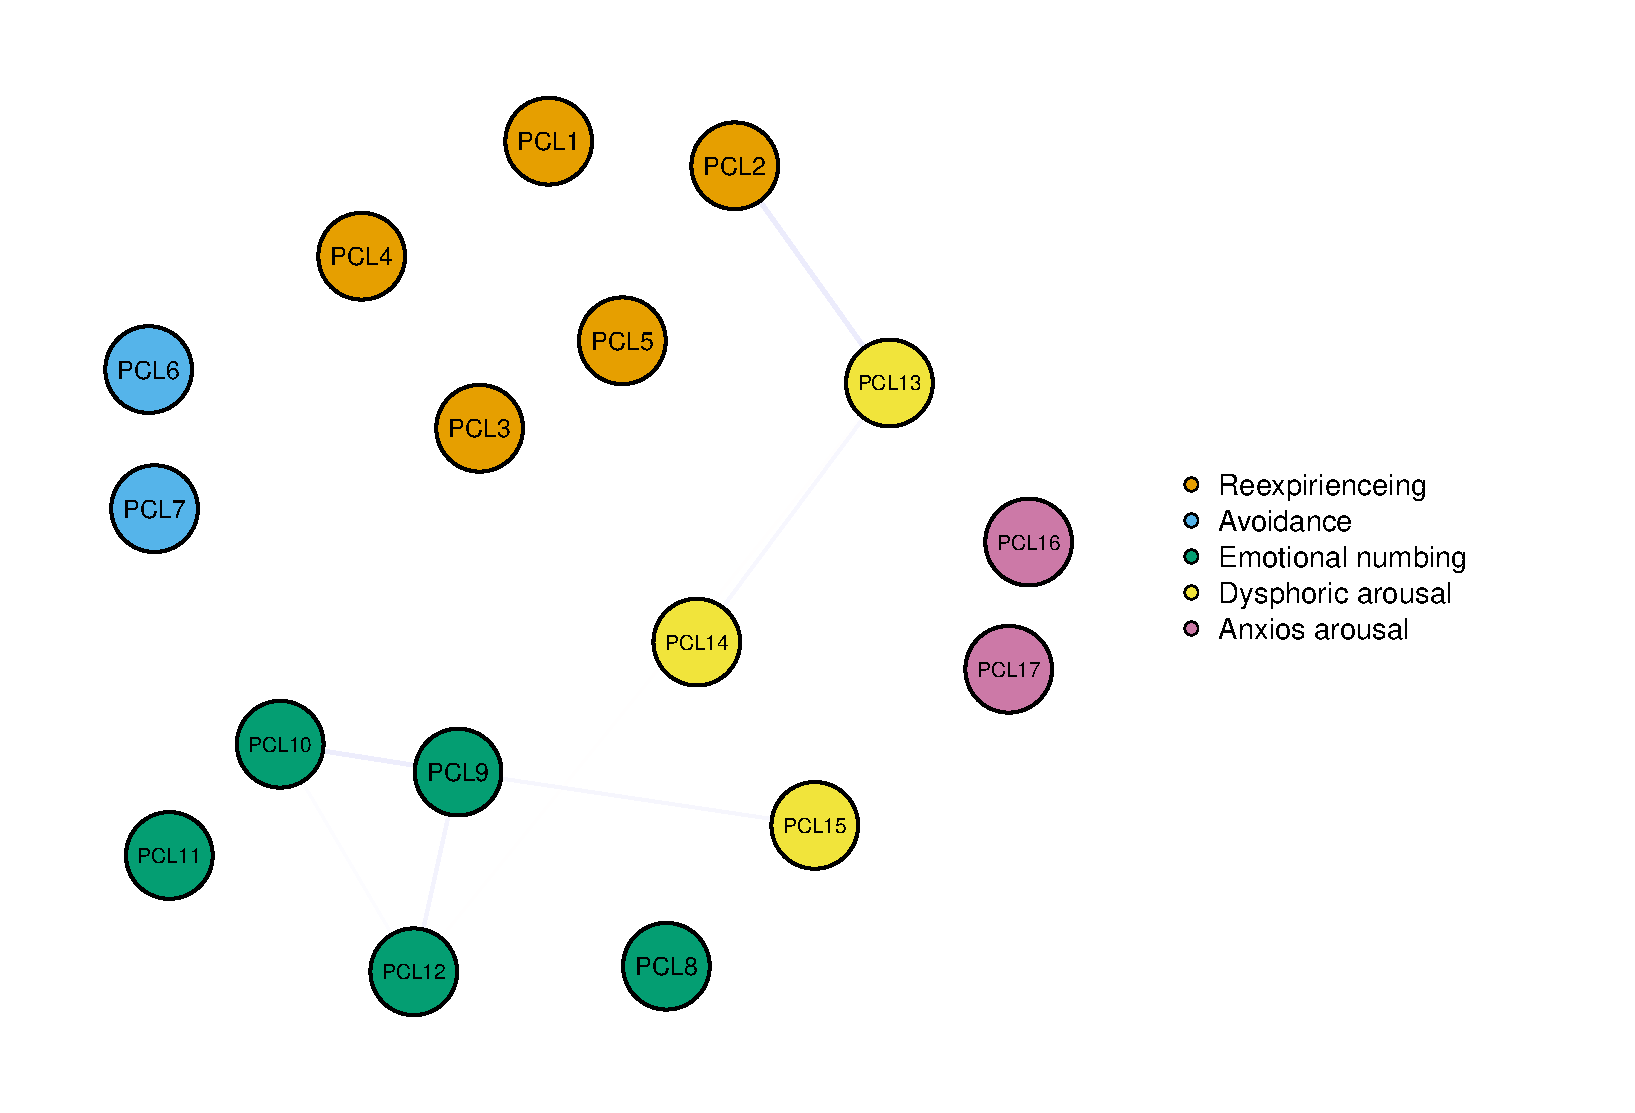
\includegraphics[width=\textwidth]{img/deltaNetworks.eps}
%\end{center}

\\
Data was analyzed using R packages: \\
bootnet $^{(Epskamp \& Fried,\ 2018)}$ \\
bnlearn $^{(Scutari,\ 2009)}$

\vfill

\begin{flushright}


\includegraphics[width=0.5\textwidth]{img/NCPTSD_Logo.png}
\hfill

\includegraphics[width=0.4\textwidth]{img/Yale.png}
\end{flushright}

}

\end{document}





